\documentclass[12pt,a4paper]{article}
\usepackage[utf8]{inputenc}
\usepackage[T1]{fontenc}
\usepackage{amsmath,amssymb}
\usepackage{graphicx}
\usepackage{float}
\usepackage{booktabs}
\usepackage{geometry}
\usepackage{xcolor}
\usepackage{hyperref}
\usepackage{fancyhdr}
\usepackage{tikz}
\usetikzlibrary{arrows.meta,positioning}
\geometry{margin=1in}
\graphicspath{{images/}}
\newcommand{\img}[2][]{\includegraphics[#1]{\detokenize{#2}}}
\pagestyle{fancy}
\fancyhf{}
\fancyfoot[C]{\thepage}
\renewcommand{\headrulewidth}{0pt}
\definecolor{headingblue}{RGB}{0,0,150}

\title{\textcolor{headingblue}{\textbf{Machine learning aided antenna optimization}\\\large Detailed Project Report}}
\author{
Pratik Kumar -- 24BML0027\\
Shruti -- 24BML0033\\
Uday Krishan Khandelwal -- 24BML0017\\[4pt]
Department of Electronics Engineering (SENSE)\\
Vellore Institute of Technology, Vellore
}
\date{\today}

\begin{document}
\begin{titlepage}
\thispagestyle{empty}
\centering
{\Large\textcolor{headingblue}{\textbf{ Machine learning aided antenna optimization}}\\[6pt]
\textcolor{headingblue}{Detailed Project Report}\\[4pt]
\normalsize Winter Semester - BECE205L\\
\normalsize Antenna and Microwave Engineering\par}
\vspace*{\fill}
{\large
Pratik Kumar -- 24BML0027\\
Shruti -- 24BML0033\\
Uday Krishan Khandelwal -- 24BML0017\\[4pt]
Department of Electronics Engineering (SENSE)\\
Vellore Institute of Technology, Vellore\\[8pt]
April 8, 2026
\par}
\vspace*{\fill}
\img[width=0.40\textwidth]{VIT_COLOURED LOGO.png}
\end{titlepage}
\newpage
\tableofcontents
\newpage

\section{Abstract}
This report presents \textit{AntennaTwin} from an antenna-engineering perspective, with emphasis on microstrip patch and dipole design, resonance behavior, impedance matching, and radiation interpretation. The workflow combines CST modeling, MATLAB Antenna Toolbox batch analysis, and OpenEMS full-wave simulation to build and validate antenna datasets before rapid surrogate-assisted exploration. Rather than centering only on software implementation, the project focuses on how electromagnetic evidence is generated and compared across tools so that design decisions remain physically meaningful. Microstrip and dipole results are interpreted through S11 trends, geometry sensitivity, and practical bandwidth/performance trade-offs. The report also outlines a path to map CST and MATLAB far-field outputs into Unity for interactive 3D radiation visualization.

\section{Introduction}
Microstrip patch and dipole antennas are fundamental in wireless systems, but they represent different electromagnetic design regimes. A patch antenna is strongly influenced by substrate properties, fringing fields, and feed topology, while a dipole is dominated by electrical length and current distribution along a conductor. Because these antennas respond differently to geometry changes, a serious design workflow must preserve physical interpretation at every stage instead of presenting outputs as generic numerical predictions.

This report frames AntennaTwin around that antenna-first philosophy. The workflow combines equation-based initialization, CST and MATLAB reference generation, and OpenEMS verification so that design decisions can be justified through resonance behavior, impedance trends, and radiation expectations.

\subsection{Microstrip Antenna}
Microstrip patch antennas are selected for compactness, planar manufacturability, and compatibility with PCB-based RF systems. Their resonant behavior depends on effective dielectric loading, patch dimensions, substrate thickness, and feed location. In practical design, even small variations in patch length or dielectric constant can shift the resonant frequency and affect return loss depth. This is why microstrip analysis in this project focuses on geometry-to-S11 sensitivity, bandwidth interpretation, and feed-dependent impedance control.

From an engineering perspective, microstrip design is a balance between size, matching quality, and fabrication constraints. The report therefore treats microstrip results not only as simulation plots, but as indicators of practical design viability under realistic substrate and frequency conditions.

\subsection{Dipole Antenna}
Dipole antennas are canonical resonant radiators and provide a clean reference for current-distribution-driven behavior. Their first-order resonance follows electrical-length principles, but practical matching still depends on conductor diameter, feed representation, and environment assumptions. In this project, dipole workflows are used to study how length and operating frequency interact with S11 minima and radiation tendencies.

Dipole analysis is valuable because it offers high interpretability: designers can directly relate resonance movement to physical length adjustments. This makes dipoles an ideal complement to microstrip studies, and together they validate that the platform supports both substrate-centric and wire-centric antenna families.

\subsection{OpenEMS}
OpenEMS is used as the full-wave verification engine in the interactive workflow. Its FDTD foundation makes it suitable for time-domain EM analysis, broadband response extraction, and repeatable computational validation under open and scriptable conditions. In this report, OpenEMS serves as the confidence layer for selected designs after initial estimation and reference comparison.

The role of OpenEMS is intentionally explicit: it answers whether a chosen geometry truly meets target resonance and matching goals under full-wave physics. This prevents over-reliance on surrogate predictions and keeps final decisions anchored in EM solver evidence.

\subsection{CST}
CST Studio Suite is used to build high-fidelity reference models and controlled parametric sweeps for both microstrip and dipole antennas. Its mature modeling and post-processing environment helps generate benchmark S11 curves and geometry-response relationships that are later used for cross-tool consistency checks.

Within this project, CST acts as a reference-quality source for antenna evidence. It helps define expected trends, supports validation of OpenEMS behavior, and strengthens confidence that model-assisted outputs remain physically consistent with established EM simulations.

\section{Problem Statement}
In antenna design practice, a major challenge is preserving physical consistency while moving between tools. For microstrip patches, small geometric or substrate changes can shift resonance significantly; for dipoles, length and feed assumptions can alter matching trends in nontrivial ways. When these analyses are performed in disconnected environments, it becomes difficult to ensure that comparisons are made under equivalent electromagnetic conditions.

Another challenge is tool-role clarity. CST, MATLAB, and OpenEMS are all capable of antenna analysis, but they are often used inconsistently. Without a clear workflow, teams may compare outputs produced with different meshing assumptions, boundary setups, or post-processing conventions. The project addresses this by defining explicit roles: CST and MATLAB for structured dataset generation and antenna insight, OpenEMS for full-wave verification in the interactive loop, and model-assisted methods only as acceleration layers grounded in those EM references.

From an antenna-engineering viewpoint, this inconsistency directly affects design quality. A resonance dip that appears acceptable in one setup may be misleading if feed definition, boundary spacing, or sweep resolution differs across tools. The central problem is therefore not only computational speed, but the absence of a unified physical interpretation layer that keeps all results comparable and decision-ready.

\section{Objectives}
The first objective is to build antenna-first workflows for microstrip patch and dipole designs, including geometry definition, resonance targeting, and S11-based validation. The second objective is to establish reliable cross-tool consistency between CST, MATLAB Antenna Toolbox, and OpenEMS so results can be compared with clear physical interpretation.

The third objective is to retain equation-level reasoning for antenna sizing and sanity checks while still prioritizing full-wave evidence for final decisions. The fourth objective is to prepare far-field outputs for interactive visualization, enabling radiation-pattern interpretation in Unity without losing traceability to CST/MATLAB/OpenEMS source simulations.

A related objective is to improve antenna decision confidence by standardizing how S11 behavior is interpreted across tools: dip location, dip depth, local bandwidth trend, and geometry sensitivity are treated as core evaluation markers for both microstrip and dipole paths.

\section{System Architecture}
The architecture is organized around antenna evidence flow rather than software complexity. CST and MATLAB Antenna Toolbox form the reference-generation side, where parametric models for microstrip and dipole antennas are created and analyzed. OpenEMS forms the deployed full-wave simulation side, where antenna behavior is recomputed under controlled numerical settings for verification. Above this, the interface layer presents inputs and outputs in antenna-centric terms: geometry, resonance frequency, S11 response, and performance metrics.

This structure supports a clear hierarchy of confidence. Analytical and catalog tools guide initial dimensions, CST/MATLAB studies provide broad reference understanding, and OpenEMS confirms selected designs in the live workflow. By preserving this order, the system avoids over-reliance on any single source and keeps interpretation anchored in electromagnetic behavior.

The architecture is therefore not only modular in software terms; it is modular in physics confidence. Early-stage tools provide exploration speed, mid-stage references provide trend reliability, and final-stage full-wave simulation provides design acceptance evidence.

\section{Methodology}
Methodology follows a fixed engineering chain so data provenance remains explicit. We first define microstrip and dipole parameter ranges and generate simulation datasets for both antenna families through controlled sweeps. For microstrip, the sweep includes patch geometry, substrate, and feed-sensitive parameters; for dipole, it includes length-centered resonant controls and geometry variants. These sweeps establish the base simulation dataset used to study resonance shift, matching behavior, and geometry sensitivity.

The second stage is MATLAB Antenna Toolbox processing, where batch runs are used to organize and export antenna responses in a structured and reusable format. MATLAB contributes rapid antenna-centric data generation and trend inspection, especially for repeatable sweep execution and quick response comparison. The third stage is CST-based dataset generation, used as a high-fidelity reference source with carefully controlled model setup and post-processing. CST outputs serve as benchmark evidence for expected S11 behavior and support cross-tool validation.

After the simulation datasets are consolidated, the model-training stage learns mapping from geometry/frequency features to response-level targets. Training is treated as an acceleration layer, not a replacement for EM physics. The trained model is then integrated into the digital twin workflow, where users can perform fast screening and still trigger OpenEMS for confidence-critical checks. In parallel, a physics-based calculator module supports equation-driven verification so users can compare numerical outputs with first-principle expectations before final design acceptance.

Method validation is based on cross-consistency: if CST, MATLAB, and OpenEMS show aligned resonance trends under equivalent geometry shifts, the workflow is treated as physically stable. Disagreements are investigated through setup assumptions (mesh density, excitation detail, boundary conditions, and frequency sweep span) before accepting outputs into the design narrative.

\begin{figure}[H]
\centering
\resizebox{\textwidth}{!}{
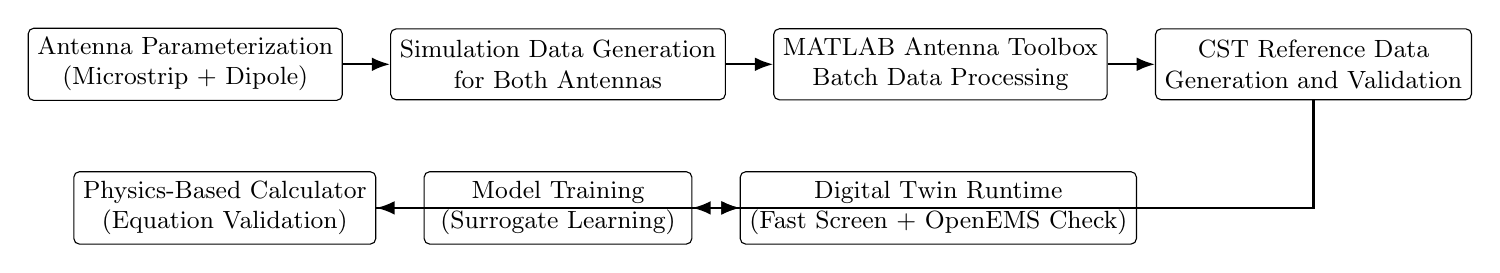
\begin{tikzpicture}[
  node distance=9mm and 6mm,
  box/.style={draw, rounded corners=2pt, align=center, font=\small, minimum height=9mm, minimum width=34mm},
  arr/.style={-Latex, thick}
]
\node[box] (p1) {Antenna Parameterization\\(Microstrip + Dipole)};
\node[box, right=of p1] (p2) {Simulation Data Generation\\for Both Antennas};
\node[box, right=of p2] (p3) {MATLAB Antenna Toolbox\\Batch Data Processing};
\node[box, right=of p3] (p4) {CST Reference Data\\Generation and Validation};

\node[box, below=of p2] (p5) {Model Training\\(Surrogate Learning)};
\node[box, right=of p5] (p6) {Digital Twin Runtime\\(Fast Screen + OpenEMS Check)};
\node[box, left=of p5] (p7) {Physics-Based Calculator\\(Equation Validation)};

\draw[arr] (p1) -- (p2);
\draw[arr] (p2) -- (p3);
\draw[arr] (p3) -- (p4);
\draw[arr] (p4) |- (p5);
\draw[arr] (p5) -- (p6);
\draw[arr] (p5) -- (p7);
\draw[arr] (p7) -- (p6);
\end{tikzpicture}
}
\caption{Methodology flow: simulation data (microstrip and dipole), MATLAB/CST generation, model training, digital twin integration, and physics-based calculation.}
\end{figure}

\section{Implementation Details}
Implementation is designed to keep antenna interpretation explicit at each step. Input panels collect physically meaningful geometry and frequency parameters for microstrip and dipole cases. The simulation path routes selected cases to OpenEMS, and output panels present S11 and related metrics in a comparable format so users can evaluate resonance quality directly.

CST and MATLAB contributions are preserved as reference artifacts rather than hidden preprocessing. Their datasets and plots are used to contextualize OpenEMS outputs and train acceleration models where appropriate. This keeps the workflow antenna-centric: every displayed value is tied back to geometry, frequency behavior, and solver/reference evidence instead of being presented as a generic software output.

Result presentation is intentionally engineered for antenna interpretation: users see parameterized geometry context with matching-relevant outputs so decisions can be made in terms of electromagnetic trade-offs, not only API success responses.

\section{Results and Demonstration}
Figures are arranged to mirror the antenna engineering lifecycle from geometry setup to radiation-aware interpretation. The sequence starts with CST and MATLAB references, proceeds to OpenEMS simulation outcomes, then shows training and prediction views, and finally closes with physics-based validation support. This order clarifies how each tool contributes to understanding microstrip and dipole behavior rather than showing disconnected screenshots.

Across sections, the key reporting criterion is interpretability of antenna behavior: whether resonance movement, matching trend, and design sensitivity can be clearly explained for both families under the same workflow logic.

\subsection{CST and MATLAB Data Generation}
This subsection documents antenna-focused reference generation. CST is used to construct physically faithful microstrip and dipole models with controlled geometry and frequency sweeps, producing baseline S11 behavior under consistent solver settings. MATLAB Antenna Toolbox is used for rapid batch evaluation and comparative trend analysis, especially useful for understanding how resonance and impedance patterns shift with parameter changes.

Using both CST and MATLAB creates complementary value: CST provides detailed model fidelity and industry-standard setup control, while MATLAB enables efficient exploratory sweeps and quick antenna insight. These references form the physical backbone used to interpret later OpenEMS and model outputs.

\begin{figure}[H]\centering\img[width=0.92\textwidth]{CST mc model.png}\caption{CST microstrip model setup.}\end{figure}
\begin{figure}[H]\centering\img[width=0.92\textwidth]{CST s11 graphs mc.png}\caption{CST microstrip S11 sweeps.}\end{figure}
\begin{figure}[H]\centering\img[width=0.92\textwidth]{dioloe cst model.jpeg}\caption{CST dipole model setup.}\end{figure}
\begin{figure}[H]\centering\img[width=0.92\textwidth]{dipole cst s11.jpeg}\caption{CST dipole S11 sweeps.}\end{figure}
\begin{figure}[H]\centering\img[width=0.92\textwidth]{matlab microstrip.png}\caption{MATLAB microstrip batch output.}\end{figure}
\begin{figure}[H]\centering\img[width=0.92\textwidth]{Dipole matlab.png}\caption{MATLAB dipole batch output.}\end{figure}

\subsection{Simulation Outputs}
Simulation outputs represent the full-wave verification stage in OpenEMS. For both microstrip and dipole designs, these results provide resonance and matching evidence directly tied to current geometry inputs. The key value here is decision confidence: OpenEMS results are used as high-fidelity anchors when selecting final dimensions or validating model-predicted trends.

In practical terms, this stage answers the core antenna question: does the selected geometry produce the intended electromagnetic response at the target frequency range? By presenting both antenna families, the report highlights that this verification logic is consistent even when physical mechanisms differ.

\begin{figure}[H]\centering\img[width=0.92\textwidth]{mc simulated design.png}\caption{Microstrip simulated design output.}\end{figure}
\begin{figure}[H]\centering\img[width=0.92\textwidth]{dipole simulated design.png}\caption{Dipole simulated design output.}\end{figure}

\subsection{Training Evidence}
Training evidence is included to show how acceleration layers are grounded in real antenna simulations. The dataset scale and structure indicate that model behavior is learned from physically generated responses rather than arbitrary synthetic values. This is important because reliable prediction depends on representative antenna geometry and frequency coverage.

The role of this stage is supportive: it enables rapid design-space screening, but it remains tied to CST/MATLAB/OpenEMS electromagnetic references. This balance preserves engineering credibility while reducing turnaround time.

\begin{figure}[H]\centering\img[width=0.92\textwidth]{1200Simulationresult.jpeg}\caption{Large-batch training/simulation evidence.}\end{figure}

\subsection{Model and Result Views}
Model and result views demonstrate how users inspect antenna behavior during interactive design. For microstrip and dipole cases, S11 and performance summaries are displayed in a common format so resonance quality and comparative trends are easy to read. This representation supports fast iteration without hiding whether outputs are model-assisted or solver-verified.

The emphasis remains antenna-centric: outputs are interpreted in terms of resonance position, match quality, and practical geometry implications, not only numerical prediction speed.

\begin{figure}[H]\centering\img[width=0.92\textwidth]{model output mc.png}\caption{Microstrip model output.}\end{figure}
\begin{figure}[H]\centering\img[width=0.92\textwidth]{model output of dipole.png}\caption{Dipole model output.}\end{figure}
\begin{figure}[H]\centering\img[width=0.92\textwidth]{mc result.png}\caption{Microstrip result metrics and S11.}\end{figure}
\begin{figure}[H]\centering\img[width=0.92\textwidth]{dipole result.png}\caption{Dipole result metrics and S11.}\end{figure}

\subsection{Physics-Calculator Views}
The physics-calculator views provide analytical context for antenna decisions. Users can navigate formulas relevant to resonance, impedance, and geometry-based estimations, then compare these expectations with CST, MATLAB, and OpenEMS outputs. This keeps theory connected to simulation and helps detect inconsistent unit usage or implausible parameter choices early.

For microstrip and dipole workflows, this layer improves interpretability by showing why a trend is expected before relying on computational outputs alone. In the current implementation, the calculator catalog contains \textbf{9 major sections}, \textbf{37 antenna/types}, and \textbf{66 detailed sub-calculators}. This breadth allows users to move from quick equations (effective wavelength, impedance relations, array factors, and gain-oriented estimates) to more specific antenna-family calculations in a single navigation path.

Calculation execution is deterministic: each calculator takes standardized inputs with unit-aware fields, evaluates closed-form or semi-empirical formulas, and returns structured outputs with units and derived metrics. This design is valuable in antenna engineering because it supports pre-simulation sizing, post-simulation plausibility checks, and quick sensitivity testing before running full-wave models.

Several representative formulas are implemented and used as first-pass engineering checks. For resonance-scale estimation, the free-space wavelength relation
\[
\lambda=\frac{c}{f}
\]
is used to initialize electrical dimensions and to verify whether a selected geometry is physically plausible at the target band. Reflection behavior is interpreted through
\[
|\Gamma|=\left|\frac{Z_L-Z_0}{Z_L+Z_0}\right|,\qquad S_{11,\mathrm{dB}}=20\log_{10}|\Gamma|
\]
so users can move directly between impedance mismatch and return-loss interpretation. For simple dipole initialization, the half-wave approximation
\[
L\approx \frac{\lambda}{2}
\]
provides a baseline before full-wave correction effects are considered. In microstrip-oriented calculations, effective dielectric behavior and guided wavelength relations are used to estimate resonant dimensions before solver-based fine tuning.

The calculation flow is intentionally consistent across all calculator types. Inputs are normalized into SI units, validated against physical ranges, and then evaluated using formula-specific expressions. Derived values are then mapped back to user-facing units and presented in a results table with explicit dimensions and symbols. This prevents hidden unit errors and makes the outputs easier to audit. In practice, users first estimate with the calculator, then run OpenEMS/CST comparisons, and finally use discrepancies to refine geometry or boundary assumptions. This loop substantially reduces blind simulation trials and improves engineering confidence, especially when microstrip substrate effects or dipole length sensitivity make design response highly nonlinear.

\begin{figure}[H]\centering\img[width=0.92\textwidth]{phys cal mc.png}\caption{Microstrip-oriented physics calculator.}\end{figure}
\begin{figure}[H]\centering\img[width=0.92\textwidth]{phys cal .png}\caption{General antenna physics calculator interface.}\end{figure}

\section{Discussion}
The key contribution is a physically grounded workflow that treats microstrip patch and dipole antennas as engineering objects first, and software entities second. By explicitly combining CST references, MATLAB antenna exploration, and OpenEMS verification, the platform improves trust in final decisions and reduces ambiguity about result origin.

Another important outcome is methodological balance. Fast predictive tools can accelerate exploration, but full-wave solvers remain central for confidence-critical steps. The report shows that this layered strategy is practical, reproducible, and better aligned with real antenna design practice than single-method pipelines.

The microstrip and dipole comparison is especially useful because it demonstrates robustness across distinct physical mechanisms. If one workflow can preserve interpretability for substrate-loaded resonators and wire radiators together, it is more likely to scale to additional antenna classes in future work.

From a strict antenna-centric perspective, the strongest result is consistency of interpretation across tools. Resonance movement with geometry variation is observable in both patch and dipole paths, and S11 trend analysis remains coherent when transitioning from MATLAB/CST references to OpenEMS verification. This reduces the risk of tool-induced misinterpretation, which is a common failure mode in multi-solver workflows.

The workflow also improves design discipline. Instead of tuning blindly for a single S11 dip, users can evaluate dip depth, resonance placement, local bandwidth behavior, and physical parameter sensitivity together. For microstrip antennas, this helps balance substrate and feed decisions with compactness; for dipoles, it improves control over electrical-length tuning and matching behavior. As a result, the platform supports engineering-grade reasoning, not only numerical output generation.

\section{Future Work}
Future work should deepen antenna analysis, especially radiation-pattern interpretation and measured-vs-simulated correlation. The highest-impact next step is a standardized far-field export pipeline across CST, MATLAB, and OpenEMS, enabling direct ingestion into Unity for interactive 3D lobe visualization, frequency sweep playback, and polarization-based comparison.

Further work should include broader parameter-space studies for microstrip and dipole variants, sensitivity analysis under fabrication tolerances, and uncertainty-aware overlays on predicted curves. These extensions will make the platform stronger not only as a software system, but as a complete antenna research and validation environment.

An additional direction is measurement integration: importing VNA-measured S11 and pattern data for selected prototypes to quantify simulation-to-hardware deviation. This would strengthen model calibration, improve trust boundaries, and make the platform directly useful for lab-to-design feedback loops.

\section{Conclusion}
AntennaTwin demonstrates that microstrip patch and dipole antenna design can be unified in a single, physically interpretable workflow without sacrificing simulation rigor. By coupling CST-based reference generation, MATLAB antenna-centric batch analysis, and OpenEMS full-wave verification, the platform keeps design decisions anchored in electromagnetic behavior rather than interface convenience.

The project confirms a practical engineering strategy: use formulas for informed initialization, use broad solver/reference datasets for trend understanding, and use OpenEMS for confidence-critical verification of selected geometries. Model-assisted acceleration remains useful, but only when tied to these EM foundations.

Overall, the report establishes a strong antenna-first baseline for future expansion, particularly toward Unity-enabled 3D radiation visualization that translates CST/MATLAB /OpenEMS far-field outputs into intuitive and review-ready electromagnetic insight.

\section*{Acknowledgment}
The authors sincerely thank \textbf{Dr Suresh Kumar T R}, Associate Professor, School of Electronics Engineering (SENSE), Vellore Institute of Technology, Vellore, for his guidance, technical feedback, and continuous support throughout the development of this project.

\begin{thebibliography}{99}
\bibitem{r1} M. Grieves and J. Vickers, ``Digital twin: Mitigating unpredictable, undesirable emergent behavior in complex systems,'' in \textit{Transdisciplinary Perspectives on Complex Systems}. Cham, Switzerland: Springer, 2017.
\bibitem{r2} F. Tao, H. Zhang, A. Liu, and A. Nee, ``Digital twin in industry: State-of-the-art,'' \textit{IEEE Trans. Ind. Informat.}, vol. 15, no. 4, pp. 2405--2415, 2019.
\bibitem{r3} A. Fuller \textit{et al.}, ``Digital twin: Enabling technologies, challenges and open research,'' \textit{IEEE Access}, vol. 8, pp. 108952--108971, 2020.
\bibitem{r4} C. A. Balanis, \textit{Antenna Theory: Analysis and Design}, 4th ed. Hoboken, NJ, USA: Wiley, 2016.
\bibitem{r5} D. M. Pozar, \textit{Microwave Engineering}, 4th ed. Hoboken, NJ, USA: Wiley, 2011.
\bibitem{r6} T. Liebig \textit{et al.}, ``openEMS -- A free and open source EC-FDTD simulation platform,'' \textit{Int. J. Numer. Model.}, vol. 32, no. 6, 2019.
\bibitem{r7} Dassault Syst\`emes, ``CST Studio Suite,'' 2024. [Online]. Available: \url{https://www.3ds.com/products/simulia/cst-studio-suite}
\bibitem{r8} A. V. Oppenheim and R. W. Schafer, \textit{Discrete-Time Signal Processing}, 3rd ed. Upper Saddle River, NJ, USA: Prentice Hall, 2009.
\bibitem{r9} S. Haykin, \textit{Adaptive Filter Theory}, 5th ed. Upper Saddle River, NJ, USA: Pearson, 2014.
\bibitem{r10} J. R. James and P. S. Hall, \textit{Handbook of Microstrip Antennas}. London, U.K.: IEE, 1989.
\bibitem{r11} C. E. Rasmussen and C. K. I. Williams, \textit{Gaussian Processes for Machine Learning}. Cambridge, MA, USA: MIT Press, 2006.
\bibitem{r12} F. Pedregosa \textit{et al.}, ``Scikit-learn: Machine learning in Python,'' \textit{J. Mach. Learn. Res.}, vol. 12, pp. 2825--2830, 2011.
\bibitem{r13} T. Chen and C. Guestrin, ``XGBoost: A scalable tree boosting system,'' in \textit{Proc. 22nd ACM SIGKDD}, 2016, pp. 785--794.
\bibitem{r14} A. Taflove and S. C. Hagness, \textit{Computational Electrodynamics: The Finite-Difference Time-Domain Method}, 3rd ed. Boston, MA, USA: Artech House, 2005.
\bibitem{r15} The MathWorks, Inc., ``Antenna Toolbox Documentation,'' 2024. [Online]. Available: \url{https://www.mathworks.com/help/antenna/}
\bibitem{r16} R. Garg, P. Bhartia, I. Bahl, and A. Ittipiboon, \textit{Microstrip Antenna Design Handbook}. Norwood, MA, USA: Artech House, 2001.
\bibitem{r17} Unity Technologies, ``Unity Manual,'' 2024. [Online]. Available: \url{https://docs.unity3d.com/Manual/}
\bibitem{r18} R. Szeliski, \textit{Computer Vision: Algorithms and Applications}, 2nd ed. Cham, Switzerland: Springer, 2022.
\bibitem{r19} FastAPI, ``FastAPI Documentation,'' 2026. [Online]. Available: \url{https://fastapi.tiangolo.com/}
\bibitem{r20} React, ``React Documentation,'' 2026. [Online]. Available: \url{https://react.dev/}
\bibitem{r21} Uvicorn, ``Uvicorn ASGI Server Documentation,'' 2026. [Online]. Available: \url{https://www.uvicorn.org/}
\bibitem{r22} A. Paszke \textit{et al.}, ``PyTorch: An imperative style, high-performance deep learning library,'' in \textit{Adv. Neural Inf. Process. Syst.}, 2019.
\end{thebibliography}
\end{document}
